%\section{Introduction}

\begin{frame}[plain]
\centering
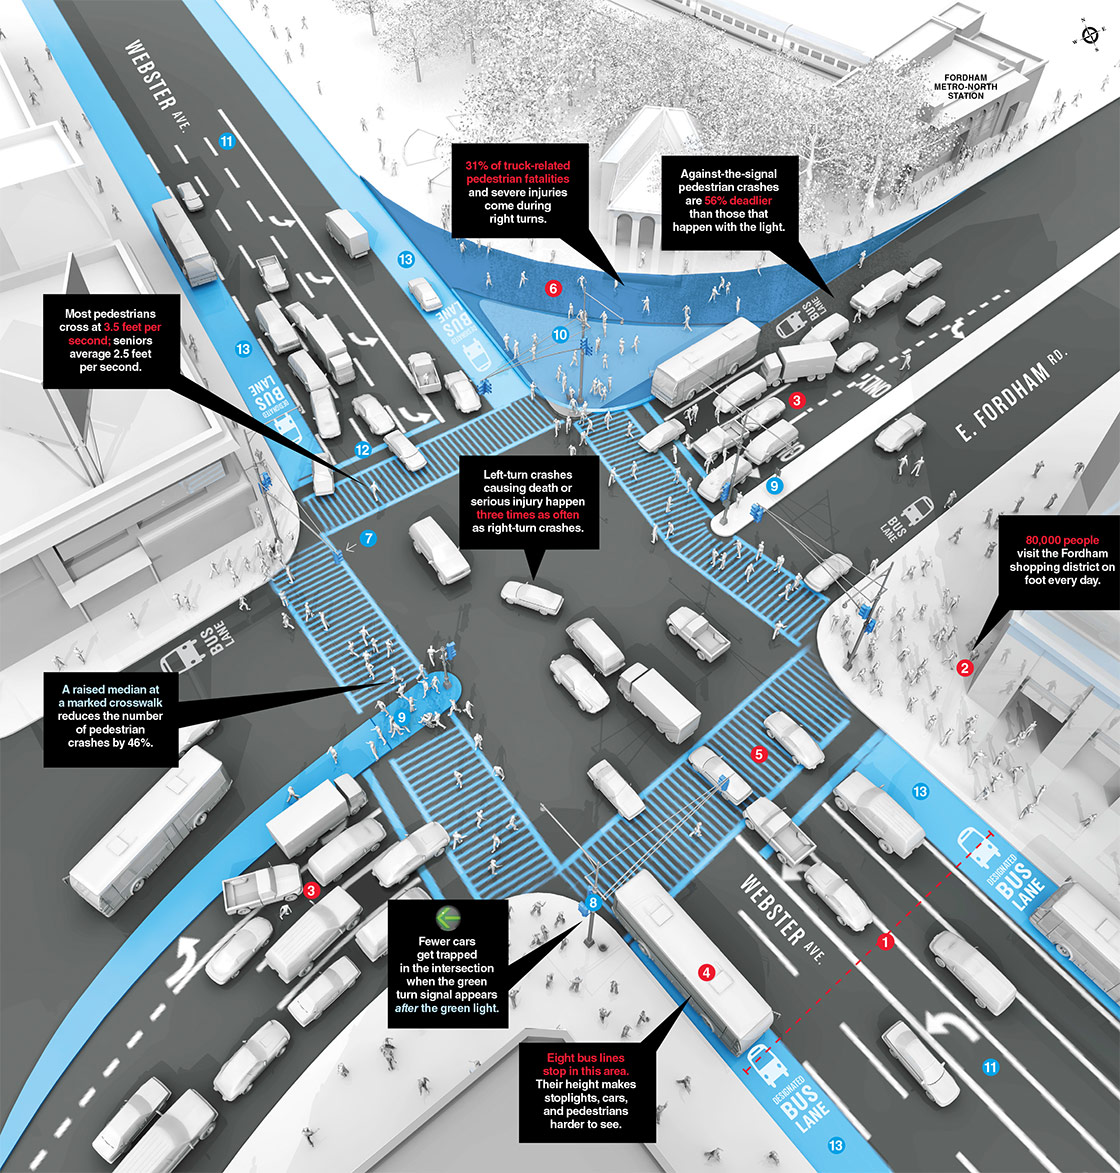
\includegraphics[width=0.75\linewidth]{diagram/nymag_intersection.jpg}

\tiny Source: \url{http://nymag.com/news/features/worst-nyc-traffic-intersections-2012-12/}
\end{frame}

\begin{frame}{Autonomous Intersections}
\begin{itemize}
\item Future roadways face congestion issues due to increasing volume
	and population density, which would likely lead to greater accident rates
\item Autonomous cars will become much more prevalent in future
\end{itemize}
\begin{block}{Objective}
Model an intelligent intersection system with a centralized controller
(as opposed to a peer-to-peer protocol) to route autonomous vehicles
\end{block}
\end{frame}

%%

\section{Objectives}

\subsection{Original Objectives}

\begin{frame}{Original Vehicle Model}
Originally, we assumed an intersection environment that contained both
human and autonomously controlled vehicles where:
\begin{itemize}
\item Human controlled vehicles respond only to \texttt{START} and 
	\texttt{STOP} commands from the controller
\item Autonomous vehicles respond to \texttt{START}, \texttt{STOP},
	\texttt{CHNG}, and \texttt{SLWDN}
\item Controller analyzes all vehicles in system and sends out commands
	to optimize throughput.
\item The intersection is a hybrid system containing both discrete and
	continuous components.
\end{itemize}
\end{frame}

\begin{frame}{Controller Knowledge}
Vehicles are equipped with embedded telemetry units that continually
notify the controller with certain information while within the
intersection environment:
\begin{itemize}
\item Current location
\item Current speed
\item Planned route
\item Entrance lane
\end{itemize}
\end{frame}

\subsection{Objective Changes}

\begin{frame}{Deviations from Original Intent}
Changes in intersection system model:
\begin{itemize}
\item Shift of focus from optimization towards correct modeling
\item Constant velocity: $a(t) = 0$
\item Changes in velocity can occur instantaneously
\item System contains autonomous vehicles only
\item Vehicle reaction to controller command is instantaneous
\item Intersection turns have no effect on velocity
\end{itemize}
\end{frame}

\begin{frame}{Rationale for Changes}
\begin{itemize}
\item Optimization of the system may be intractable for application
\item Human-controlled vehicles would be a rarity in the described system
\item Constant velocity model reasonable within limited intersection distances
\item Limitations with dynamic actor instantiation in Ptolemy modeling
\item Learning curve involved with modeling tool (Ptolemy)
\end{itemize}
\end{frame}

\begin{frame}{Modeling Objectives}
Let $c$ denote the event in which a collision event has occurred at time $t$,
and let $e$ denote the event in which car $v$ has entered a route within
the intersection.
\begin{itemize}
\item Safety: $\forall t: G(\neg c)$
\item Fairness: $\forall v: F e$
\end{itemize}
\end{frame}
